\documentclass{article}
\usepackage[margin=0.75in]{geometry}
\usepackage{makecell}
\usepackage{longtable}
\usepackage{amsmath, amssymb}
\usepackage{listings}
\usepackage{xcolor}
\usepackage{tikz}
\usepackage{tcolorbox}
\tcbuselibrary{skins, breakable}

\lstdefinestyle{bashconsole}{
    backgroundcolor=\color{black!5},
    basicstyle=\ttfamily\color{black},
    keywordstyle=\color{blue}\bfseries,
    commentstyle=\color{green!70!black},
    stringstyle=\color{red!70!black},
    numberstyle=\tiny\color{gray},
    breaklines=true,
    frame=single,
    rulecolor=\color{black!20},
    xleftmargin=0.5cm,
    numbers=left,
    numbersep=5pt,
    literate={\$}{{\textcolor{blue}{\$}}}1,
    showstringspaces=false,
    upquote=true,
}

\usetikzlibrary{shapes.geometric, arrows}

\tikzstyle{startstop} = [rectangle, rounded corners, minimum width=3cm, minimum height=1cm,text centered, draw=black, fill=red!30]
\tikzstyle{process} = [rectangle, minimum width=3cm, minimum height=1cm, text centered, draw=black, fill=orange!30]
\tikzstyle{decision} = [diamond, aspect=2, text centered, draw=black, fill=green!30]
\tikzstyle{arrow} = [thick,->,>=stealth]

\definecolor{mauve}{rgb}{0.58,0,0.82}

\lstdefinelanguage{assembly}{
  alsoletter={.}, % allow dots in keywords
  alsodigit={0x}, % hex numbers are numbers too!
  morekeywords=[1]{ % instructions
    load, loadu, loadw, zero, store,
    add, sub, mul, div, idiv,
    cmp, jmp, b, beq, bne, bge, bgt, ble, blt, bz, bnz,
    not, and, or, xnor, shr, shl,
    push, pushw, pop, popw,
    call, syscall, ret,
    nop, exit
  },
  morekeywords=[2]{
    \%define, \%end, \%include, \%macro, \%rm, \%stop
  },
  morekeywords=[3]{
    \$ip, \$sp, \$fp, \$flag, \$ret, \$zero,
    r1, \$r2, \$r3, \$r4, \$r5, \$r6, \$r7, \$r8, \$r9, \$r10, \$r11, \$r12, \$r13, \$r14, \$r15, \$r16,
    \$s1, \$s2, \$s3, \$s4, \$s5, \$s6, \$s7, \$s8
  },
  commentstyle=,
  morecomment=[l]{;},   % mark ; as line comment start
  morestring=[b]",      % mark " as string start/end
  morestring=[b]'       % also mark ' as string start/end
  % listings sonderzeichen (for german weirdness)
}

\lstdefinestyle{assembly}{
  language=assembly,
  basicstyle=\ttfamily,
  breaklines=true,
  commentstyle=\itshape\color{green!50!black},
  keywordstyle=[1]\color{blue!80!black},
  keywordstyle=[2]\color{orange!80!black},
  keywordstyle=[3]\color{red!50!black},
  stringstyle=\color{mauve},
  identifierstyle=\color{teal},
  frame=l,
  tabsize=2,
  showstringspaces=false
}

\setlength{\parindent}{0pt}

\title{Assembler Documentation}
\author{Ruben Saunders}
\date{August 2024}

\begin{document}

\maketitle

\section{Overview}

The assembler takes \textbf{one} assembly source file and produces a binary output file, which may be executed by the processor.

\textbf{Disclaimer}: The assembly language designed for this project is relatively simplistic.
Its goal is to allow for full operation of the processor with minimal-to-no additional features.
This is so focus can be given to the development of a high-level language.

\subsection{Command-Line Interface}

The assembler executable is called as follows:

\medskip
\begin{lstlisting}[style=bashconsole]
$ ./assembler <input_file> -o <output_file> [flags]
\end{lstlisting}

The output file is provided after the \texttt{-o} flag.
The following optional flags are available:
\begin{itemize}
    \item \texttt{-d}: enables debug mode.
    In this mode, detailed results from each step are output to the console.
    \item \texttt{--no-pre-process}: skips the pre-processing step.
    \item \texttt{--no-compile}: skips the compilation step.
    \textbf{Note} in this case, the \texttt{-o} flag is not compulsory.
    \item \texttt{-p <filename>}: writes the post-processed source to \texttt{filename}.
\end{itemize}

\subsection{Process Flow}

\bigskip
\begin{tcolorbox}[enhanced, breakable, parbox=false, colback=white]
    \begin{center}
    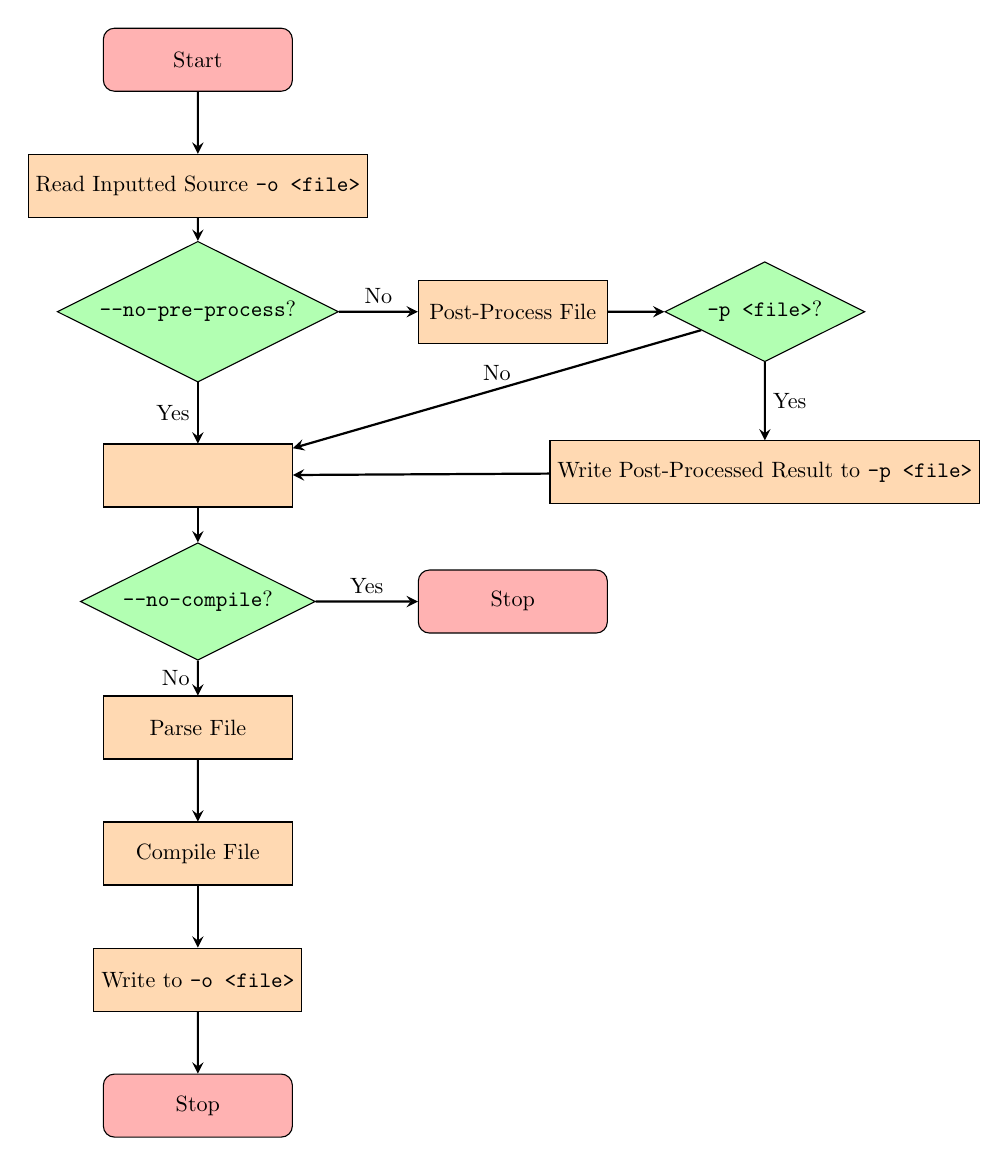
\begin{tikzpicture}[node distance=2cm, scale=0.8, transform shape]
        \node (start) [startstop] {Start};
        \node (process1) [process, below of=start] {Read Inputted Source \texttt{-o <file>}};
        \node (decision1) [decision, below of=process1] {\texttt{--no-pre-process}?};

        \node (process2) [process, right of=decision1, xshift=3cm] {Post-Process File};
        \node (decision2) [decision, right of=process2, xshift=2cm] {\texttt{-p <file>}?};
        \node (process3) [process, below of=decision2, yshift=-0.55cm] {Write Post-Processed Result to \texttt{-p <file>}};

        \node (process4) [process, below of=decision1, yshift=-0.6cm] {};
        \node (decision3) [decision, below of=process4] {\texttt{--no-compile}?};

        \node (stop1) [startstop, right of=decision3, xshift=3cm] {Stop};

        \node (process5) [process, below of=decision3] {Parse File};
        \node (process6) [process, below of=process5] {Compile File};
        \node (process7) [process, below of=process6] {Write to \texttt{-o <file>}};
        \node (stop2) [startstop, below of=process7] {Stop};
    
        \draw [arrow] (start) -- (process1);
        \draw [arrow] (process1) -- (decision1);
        \draw [arrow] (decision1) -- node[anchor=south] {No} (process2);
        \draw [arrow] (decision1) -- node[anchor=east] {Yes} (process4);
        \draw [arrow] (process2) -- (decision2);
        \draw [arrow] (decision2) -- node[anchor=west] {Yes} (process3);
        \draw [arrow] (decision2) -- node[anchor=south] {No} (process4);
         \draw [arrow] (process3) -- (process4);
         \draw [arrow] (process4) -- (decision3);
         \draw [arrow] (decision3) -- node[anchor=south] {Yes} (stop1);
         \draw [arrow] (decision3) -- node[anchor=east] {No} (process5);
         \draw [arrow] (process5) -- (process6);
         \draw [arrow] (process6) -- (process7);
         \draw [arrow] (process7) -- (stop2);
    \end{tikzpicture}
    \end{center}
\end{tcolorbox}

\section{Pre-Processor}

The pre-processor runs prior to compilation.
It modifies the source file's contents before being passed to the compiler.

Core to the pre-processor are \textit{directives}, which are commands to the pre-processor.
Directives are prefixed with a percent (\%) symbol.

\medskip
\begin{longtable}{|c|l|l|}
    \hline
    \textbf{Directive} & \textbf{Signature} & \textbf{Description} \\
    \hline
    Constant Definition & \texttt{\%define <name> <value>} & \makecell[l]{(Re-)Defines a constant \texttt{name} with the given value.\\%
    \textbf{Note} \texttt{<value>} extends to the end of the line.\\%
    \textbf{Note} the start is trimmed of whitespace, but trailing\\%
    whitespace is preserved.} \\
    \hline
    End & \texttt{\%end} & Marks the end of a macro definition. \\
    \hline
    Include File & \texttt{\%include [lib:]<path>} & \makecell[l]{Reads the file contents of \texttt{<path>} and inserts into source.\\%
    \textbf{Note} the \texttt{lib:} prefix navigates to the library directory.} \\
    \hline
    Macro Definition & \texttt{\%macro <name> [<args ...>]} & \makecell[l]{(Re-)Defines a macro with the given name and arguments.\\%
    See the below section for more information.} \\
    \hline
    Ignore Line & \texttt{\%rm <data ...>} & This removes the line from the source. \\
    \hline
    Halt \& Cut & \texttt{\%stop} & \makecell[l]{Stops the pre-processor at this line.\\%
    This and all lines succeeding it are removed from the source.} \\
    \hline
\end{longtable}

\subsection{Macros}

Macros are like pre-processor functions, and may be used to for meta-programming purposes and simplifying code.
Macros have a name and a number of arguments.
The macro's body extends from after the newline to the next \texttt{\%end} directive.
Note that arguments do not have types, as types do not exist at this level.

When referenced, the data after the macro name are split by whitespace and passed position-wise to the arguments.
The argument names are substituted with their values in the macro's body before the reference is itself substituted by this body.

For example,

\begin{lstlisting}[style=assembly]
%macro inc reg
    add reg, reg, 1
%end

inc $r1
\end{lstlisting}

is replaced with

\begin{lstlisting}[style=assembly]
add $r1, $r1, 1
\end{lstlisting}

\section{Assembly Syntax}

After pre-processing is the parsing \& compilation stage.
This section will cover the syntax of the assembly language.
Note that some syntax, such as addressing modes, is covered in the processor documentation document.

The parser reads the source line-by-line, top-to-bottom.
The most common syntax is:

\begin{lstlisting}[style=assembly]
[label:] <mnemonic>[conditional][.datatype] [args ...] [; comment]
\end{lstlisting}

Alternatively, the following is used to load data:

\begin{lstlisting}[style=assembly]
.<type> <data ...>
\end{lstlisting}

Each sub-section will go over the key components identifier in each.

\subsection{Labels}

Labels are defined at start of a line, starting with an alphabetic character or an underscore and any number of alphanumeric characters or underscores, and finally a colon.

A label is a symbol name tied to a memory address; when defined, a label adopts the value of the byte offset in memory.
When refenced, 

\end{document}
